\clearpage{}

\pagestyle{body}

\chapter{First chapter}
\label{chap:first}

\thesisepisrcyear{What is the meaning of life?}{John Doe}{Thoughts}{1971}

\chapterintrobox{This is the introduction paragraph.}

\section{First section}
\label{sec:chap-first-first}

\subsection{First subsection}
\label{subsec:chap-first-first}

\lettrine{T}{his} is the first chapter of the \gls{phd} thesis.\footnote{Hyperlinks are coloured for highlighting/debugging purposes. Colours can be removed using the \texttt{\textbackslash{hidelinks}} option.}
That acronym entry is italicised as being jargon, as opposed to other acronyms such as \gls{2d} and \gls{3d}.
Non eram nescius, Brute, cum, quae summis ingeniis exquisitaque doctrina philosophi Graeco sermone tractavissent, ea Latinis litteris mandaremus, fore ut hic noster labor in varias reprehensiones incurreret.
Nam quibusdam, et iis quidem non admodum indoctis, totum hoc displicet philosophari.
Quidam autem non tam id reprehendunt, si remissius agatur, sed tantum studium tamque multam operam ponendam in eo non arbitrantur.
Erunt etiam, et ii quidem eruditi Graecis litteris, contemnentes Latinas, qui se dicant in Graecis legendis operam malle consumere.
Postremo aliquos futuros suspicor, qui me ad alias litteras vocent, genus hoc scribendi, etsi
sit elegans, personae tamen et dignitatis esse negent.

We define the \textquote{frequency} \(\gls{s_f} = 1/\gls{s_t}\).
There is a famous result shown in \cref{eq:chap-first-eq1},
\begin{equation}
  \pd{\phi}{x}\pd{\phi}{y} \neq \cpd{\phi}{x}{y}
  \label{eq:chap-first-eq1}
\end{equation}
and another one in \cref{eq:chap-first-eq2},
\begin{equation}
  \abs{x + y} \leq \abs{x} + \abs{y}
  \label{eq:chap-first-eq2}
\end{equation}

We show some data in \cref{tab:chap-first-data}, and a sketch in \cref{fig:chap-first-sketch}.
We use previously published results in this work such as those of \textcite{villani2009}.
Other works should also be kept in mind \autocite{feynman-phd,nash1950}.
For further details, the reader is referred to \cref{appx:first}.
\begin{table}
  \caption{Some data in a table}
  \begin{tabular}{lrr}
    \toprule
    Class & Number & Age \\
    \midrule
    A     & 20     & 43 \\
    B     & 26     & 30 \\
    C     & 42     & 24 \\
    \bottomrule
  \end{tabular}
  \label{tab:chap-first-data}
\end{table}
\begin{figure}
  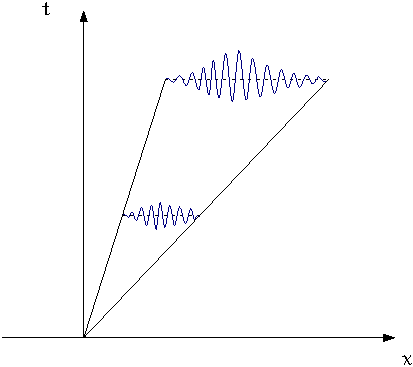
\includegraphics{chap_first_sketch}
  \caption[A sketch, with some symbols]{A sketch, with some symbols: A (\protect\blackline), B (\protect\blueline), C (\protect\blackcross) and D (\protect\blacktriangle)}
  \label{fig:chap-first-sketch}
\end{figure}

As Galileo Galilei said,

\begin{displayquote}
  The sun, with all the planets revolving around it, and depending on it, can still ripen a bunch of grapes as though it had nothing else in the universe to do.
\end{displayquote}